\section{Teoremas diretos e agendas de altura}
\label{sec:direct-height}

O paradigma de teoremas diretos e inversos tem antecedentes tanto na
aproximação por splines e em espaços de Besov quanto na aproximação por funções
racionais \citep{petrushev1988,petrushevpopov1987}. Nesta última expressão,
``racional'' significa quociente de polinômios, e não a aritmética dos
coeficientes da biblioteca; o elemento novo desta seção é acompanhar
explicitamente a altura desses coeficientes.

Fixe a raiz diádica $K=J_{k_0,m_0}$ e escreva $L=|K|=2^{-k_0}$. Para
$f\in C(K)$, defina
\begin{align}
 \omega_1(f,t)_{\infty,K}
 &=\sup_{\substack{0<h\le t\\x,x+h\in K}}
   |f(x+h)-f(x)|,\label{eq:first-modulus}\\
 \omega_2(f,t)_{\infty,K}
 &=\sup_{\substack{0<h\le t\\x,x+2h\in K}}
   |f(x+2h)-2f(x+h)+f(x)|.
 \label{eq:second-modulus-direct}
\end{align}
Para $0<s<2$ e $0<q\le\infty$, usaremos a caracterização diádica equivalente da
quase-norma de Besov
\begin{equation}
 \|f\|_{B^s_{\infty,q}(K)}^*
 :=\|f\|_{\infty,K}
 +\left\|\bigl(2^{rs}\omega_2(f,L2^{-r})_{\infty,K}
           \bigr)_{r\ge0}\right\|_{\ell^q}.
 \label{eq:dyadic-besov-norm}
\end{equation}
Ela é equivalente à definição integral com medida $\dd t/t$; essa
discretização é clássica e decorre das desigualdades de escala do módulo de
suavidade \citep{devorelorentz1993,devorepopov1988}.

Também será usada a desigualdade de Whitney de ordem dois
\citep{whitney1957,devore1998}: existe uma
constante universal $C_W$ tal que, em todo subintervalo $J\subset K$,
\begin{equation}
 \inf_{\ell\ \text{afim}}\|f-\ell\|_{\infty,J}
 \le C_W\omega_2(f,|J|)_{\infty,J}.
 \label{eq:whitney-direct}
\end{equation}
Como o interpolador nos extremos reproduz funções afins e tem norma de
operador $1$, seu erro é no máximo duas vezes o lado direito.

Ponha
\begin{equation}
 \nu_s=\max\{1,s\},
 \qquad C_K=4(k_0+|m_0|+2).
 \label{eq:height-schedule-constants}
\end{equation}

\subsection{Racionalização com denominador comensurável}

A prova precisa acompanhar também primeiras diferenças. A desigualdade de
Marchaud de ordens um e dois
\citep{devorelorentz1993,lorentz1996} implica, para $0<t\le L/2$,
\begin{equation}
 \omega_1(f,t)_{\infty,K}
 \le C_s\|f\|_{B^s_{\infty,\infty}(K)}^*
 \begin{cases}
  (t/L)^s,&0<s<1,\\
  (t/L)\log(eL/t),&s=1,\\
  t/L,&1<s<2.
 \end{cases}
 \label{eq:marchaud-regimes}
\end{equation}
Essa é exatamente a informação necessária para limitar a inclinação quando
o denominador disponível é menor que o inverso da malha.

\begin{lemma}[Jackson racional com altura explícita]
\label{lem:rational-jackson-height}
Seja $f\in B^s_{\infty,\infty}(K)$, $R=\|f\|_\infty$. Existe
$n_0=n_0(f,K,s)$ tal que, para toda potência de dois $n=2^r\ge n_0$ e todo
inteiro
\[
 H\ge\max\{C_Kn^{\nu_s},16(R+1)\}
\]
que satisfaça
\begin{equation}
 H\ge\max\{2,k_0+r+1,
      \max_{0\le j<n}|2^rm_0+j|+1\},
 \label{eq:height-geometry-condition}
\end{equation}
existe $g_{n,H}\in\Aclass_{n,H}(K)$ tal que
\begin{equation}
 \|f-g_{n,H}\|_\infty
 \le 2C_W\omega_2(f,L/n)_{\infty,K}
      +\frac{C(R+1)}{H},
 \label{eq:rational-jackson-height}
\end{equation}
onde $C$ é absoluto e $C_W$ é a constante de Whitney.

Além disso, existe $A_{K,s}\ge1$, independente de $f$, com a seguinte versão
uniforme. Se $B\ge1$, $\|f\|_{B^s_{\infty,\infty}(K)}^*\le B$, $n=2^r\ge2$
e
\begin{equation}
 H\ge A_{K,s}(B+1)n^{\nu_s},
 \label{eq:uniform-ball-height-threshold}
\end{equation}
então todas as conclusões anteriores valem sem limiar dependente de $f$ e com
o último termo de \eqref{eq:rational-jackson-height} igual a
$8(B+1)/H$. A constante $A_{K,s}$ também torna automática a condição
geométrica \eqref{eq:height-geometry-condition}.
\end{lemma}

\begin{proof}
Escolha a maior potência de dois $Q$ tal que
$8(R+1)Q\le H$. Para $H\ge16(R+1)$,
\begin{equation}
 \frac{H}{16(R+1)}<Q\le\frac{H}{8(R+1)}.
 \label{eq:Q-window}
\end{equation}
Nos nós $t_j=\inf K+jL/n$, use as grades alternadas
\[
 G_j=\frac1Q\left(\mathbb Z+\frac{j\bmod2}{2}\right)
\]
e escolha $v_j\in G_j$ mais próximo de $f(t_j)$; se os dois vizinhos da grade
forem equidistantes, escolha o menor. Então
$|v_j-f(t_j)|\le(2Q)^{-1}$ e $v_j\ne v_{j+1}$. Escrevendo
$v_j=b_j/(2Q)$ com $b_j\equiv j\pmod2$, obtém-se
\begin{equation}
 |b_j|\le2QR+1.
 \label{eq:general-b-bound}
\end{equation}
Na célula $J_{k_0+r,2^rm_0+j}$, os parâmetros são
\begin{equation}
 y_{0,j}=\frac{b_j+b_{j+1}}{4Q},
 \qquad
 s_j=2^{k_0+r}\frac{b_{j+1}-b_j}{2Q}.
 \label{eq:general-atom-parameters}
\end{equation}
A janela \eqref{eq:Q-window} e \eqref{eq:general-b-bound} dão
$\height(y_{0,j})\le H$. Como $b_{j+1}-b_j$ é ímpar, não há cancelamento
oculto com $2Q$. Se $2^{k_0+r}\le2Q$, a fração reduzida de $s_j$ tem
numerador $b_{j+1}-b_j$ e denominador $2Q/2^{k_0+r}$; a cota grosseira
$|b_{j+1}-b_j|\le4QR+2$ prova $\height(s_j)\le H$ após um aumento absoluto
do limiar inicial.

Se $2^{k_0+r}>2Q$, a inclinação é inteira e
\begin{equation}
 |s_j|
 \le \frac nL\left(\omega_1(f,L/n)+\frac1Q\right).
 \label{eq:slope-marchaud-bound}
\end{equation}
Nos três regimes de \eqref{eq:marchaud-regimes}, o primeiro termo é limitado,
respectivamente, por
\[
 C_{K,s}\|f\|_{B^s_{\infty,\infty}}^*n^{1-s},\qquad
 C_{K}\|f\|_{B^1_{\infty,\infty}}^*\log(en),\qquad
 C_{K,s}\|f\|_{B^s_{\infty,\infty}}^*;
\]
o segundo é $O((R+1)n/H)$. Com o coeficiente fixo da primeira parte, essas
quantidades ficam abaixo de $H$ quando $n\ge n_0(f,K,s)$. Se a norma é no
máximo $B$, as desigualdades elementares
$n^{1-s}\le n$, $\log(en)\le2n$ e $1\le n^{\nu_s}$, juntamente com
\eqref{eq:uniform-ball-height-threshold}, dão a mesma conclusão para todo
$n\ge2$ após escolher $A_{K,s}$ suficientemente grande. Como
\[
 k_0+r+1\le C_Kn,\qquad
 \max_{0\le j<n}|2^rm_0+j|+1\le(|m_0|+1)n+1,
\]
essa escolha também cobre a geometria. Logo cada peça pertence a
$\Library_H$ em ambas as versões.

Se $P_nf$ é o interpolante dos valores exatos nos mesmos nós, a estimativa
de Whitney \eqref{eq:whitney-direct} dá
\[
 \|f-P_nf\|_\infty
 \le2C_W\omega_2(f,L/n)_{\infty,K}.
\]
A diferença entre os dois interpolantes é, em cada célula, uma combinação
convexa dos erros nodais e não excede $(2Q)^{-1}$. Usando
\eqref{eq:Q-window}, esse termo é estritamente menor que
$8(R+1)/H\le8(B+1)/H$ na versão uniforme. Isso prova as duas afirmações.
\end{proof}

\subsection{Imersão direta sem o expoente espúrio}

Para $\kappa\ge0$, defina a agenda inteira
\begin{equation}
 H_{s,\kappa}(N)
 =\left\lceil C_K(N+1)^{\nu_s}
        [\log(eN)]^\kappa\right\rceil.
 \label{eq:corrected-height-schedule}
\end{equation}
Ela é não decrescente e satisfaz a obstrução geométrica de
\eqref{eq:height-geometry-condition} em toda malha uniforme com no máximo
$N$ folhas.

\begin{theorem}[direção direta com altura aritmética]
\label{thm:direct-besov-height}
Se $0<s<2$, então as seguintes inclusões de conjuntos valem:
\begin{align}
 B^s_{\infty,\infty}(K)
 &\subset
 \mathscr A^s_\infty(\Library,H_{s,0}),
 \label{eq:direct-endpoint}\\
 B^s_{\infty,q}(K)
 &\subset
 \mathscr A^s_q(\Library,H_{s,0}),
 &&0<q<\infty,\qquad 0<s<1,
 \label{eq:direct-subcritical}\\
 B^s_{\infty,q}(K)
 &\subset
 \mathscr A^s_q(\Library,H_{s,\kappa}),
 &&0<q<\infty,\qquad 1\le s<2,\qquad\kappa>1/q.
 \label{eq:direct-critical-log}
\end{align}
Em particular, para $s\ge1$, o endpoint $q=\infty$ admite
$H(N)=O_K(N^s)$; para $q<\infty$, basta acrescentar um fator logarítmico
crítico. Como
alternativa sem logaritmo, para qualquer $\eta>0$ pode-se substituir
$H_{s,\kappa}$ em \eqref{eq:direct-critical-log} por
\begin{equation}
 \widetilde H_{s,\eta}(N)
 =\left\lceil C_K(N+1)^{\max\{1,s+\eta\}}\right\rceil.
 \label{eq:polynomial-slack-schedule}
\end{equation}
\end{theorem}

\begin{proof}
Seja $n=2^r$. Para $r$ suficientemente grande, o
\cref{lem:rational-jackson-height} aplicado a
$H=H_{s,\kappa}(n)$ dá
\begin{equation}
 n^s e_n^{\Library,H}(f)
 \le C n^s\omega_2(f,L/n)_{\infty,K}
     +C_f\frac{n^s}{H_{s,\kappa}(n)}.
 \label{eq:direct-sequence-bound}
\end{equation}
Um número finito de escalas iniciais não afeta pertinência a $\ell^q$. O
primeiro termo do lado direito pertence a $\ell^q$ por
\eqref{eq:dyadic-besov-norm}. Se $s<1$, o segundo decai geometricamente como
$n^{s-1}$. Se $s\ge1$, ele é $O(r^{-\kappa})$, pois
$\log(en)\asymp r$; pertence a $\ell^q$ quando $\kappa q>1$ e é limitado
quando $q=\infty$ e $\kappa=0$. A agenda
\eqref{eq:polynomial-slack-schedule} produz, em vez disso, o fator
$n^{-\eta}$. O \cref{thm:dyadic-rate-equivalence} transfere as conclusões
das potências de dois para todos os orçamentos $N$.
\end{proof}

O limiar $n_0(f,K,s)$ do primeiro enunciado não impede uniformidade sobre
conjuntos normados: a segunda parte do
\cref{lem:rational-jackson-height} permite calibrar uma única agenda para uma
bola inteira. A formulação quantitativa seguinte é deliberadamente em termos
de bolas, porque o funcional de taxa não é homogêneo sobre escalares reais
pela \cref{prop:nonhomogeneous-functional}.

\begin{corollary}[imersões quantitativas uniformes sobre bolas]
\label{cor:uniform-besov-ball-embedding}
Para $B\ge1$ e $\kappa\ge0$, defina
\begin{equation}
 \widehat H_{s,\kappa}^{[B]}(N)
 =\left\lceil A_{K,s}(B+1)(N+1)^{\nu_s}
        [\log(eN)]^\kappa\right\rceil .
 \label{eq:ball-calibrated-height-schedule}
\end{equation}
Existem constantes independentes de $B$ e de $f$ tais que
\begin{align}
 \sup_{\|f\|_{B^s_{\infty,\infty}(K)}^*\le B}
 \mathfrak a_{s,\infty}^{\Library,
       \widehat H_{s,0}^{[B]}}(f)
 &\le C_{K,s}(B+1), &&0<s<2,\label{eq:uniform-ball-endpoint}\\
 \sup_{\|f\|_{B^s_{\infty,q}(K)}^*\le B}
 \mathfrak a_{s,q}^{\Library,
       \widehat H_{s,0}^{[B]}}(f)
 &\le C_{K,s,q}(B+1), &&0<s<1,\quad0<q<\infty,
 \label{eq:uniform-ball-subcritical}\\
 \sup_{\|f\|_{B^s_{\infty,q}(K)}^*\le B}
 \mathfrak a_{s,q}^{\Library,
       \widehat H_{s,\kappa}^{[B]}}(f)
 &\le C_{K,s,q,\kappa}(B+1),
 &&1\le s<2,\quad0<q<\infty,\quad\kappa>1/q.
 \label{eq:uniform-ball-critical}
\end{align}
Assim, cada bola de Besov é enviada uniformemente a uma bola do funcional de
taxa sob uma única agenda, sem qualquer limiar dependente da função.
\end{corollary}

\begin{proof}
Para $n=2^r\ge2$, a versão uniforme do
\cref{lem:rational-jackson-height} fornece
\[
 n^s e_n^{\Library,\widehat H}(f)
 \le C_{K,s}n^s\omega_2(f,L/n)_{\infty,K}
 +C_{K,s}\frac{n^s}{n^{\nu_s}[\log(en)]^\kappa}.
\]
O primeiro termo tem norma $\ell^q$ limitada por $C_{K,s}B$ na
caracterização \eqref{eq:dyadic-besov-norm}. O segundo é limitado para
$q=\infty$; é geometricamente somável se $s<1$ e $\kappa=0$; e pertence a
$\ell^q$ se $s\ge1$ e $\kappa q>1$. A escala $N=1$ é limitada por
$\|f\|_\infty\le B$. A equivalência diádica do
\cref{thm:dyadic-rate-equivalence} conclui as três cotas.
\end{proof}

\begin{remark}[o papel do índice $q$]
\label{rem:q-height-role}
O denominador comum determina o expoente aritmético e o índice $q$ determina
a somabilidade. Uma quantização de ordem
$H(N)^{-1}=N^{-s}$ deixa o termo normalizado $N^se_N$ apenas limitado; isso
é suficiente para o supremo, mas a sequência constante não pertence a
$\ell^q$ para $q<\infty$. O fator $[\log(eN)]^\kappa$, $\kappa>1/q$, torna
\[
 \sum_{N\ge2}\frac1{N[\log(eN)]^{\kappa q}}<\infty.
\]
Esse fator logarítmico é suficiente no argumento uniforme por
racionalização.
\end{remark}

\subsection{Endpoint quadrático e agudeza da agenda construtiva}

\begin{corollary}[endpoint $C^2$]
\label{cor:c2-direct-endpoint}
Na raiz $K=[0,1]$, seja
$\mathcal F_{R,M}=\{f\in C^2[0,1]:\|f\|_\infty\le R,
\|f''\|_\infty\le M\}$ e
\[
 C_H=\max\{4(R+1),\,2(4R+M/2+1)\}.
\]
Com $H_2(N)=\lceil C_HN^2\rceil$,
\begin{equation}
 \sup_{f\in\mathcal F_{R,M}}
 \mathfrak a_{2,\infty}^{\Library,H_2}(f)
 \le\max\left\{R,\frac{M+4}{2}\right\}.
 \label{eq:c2-direct-endpoint}
\end{equation}
As montagens que realizam a cota para $N\ge2$ usam
$O_{R,M}(N\log(2N))$ bits nos três formatos prefix-free do
\cref{thm:coding-formats}.
\end{corollary}

\begin{proof}
A \cref{thm:joint-budget} fornece, para todo $N\ge2$,
\[
 E_{N,\lceil C_HN^2\rceil}^{\Library}(f)_\infty
 <\frac{M+4}{2N^2}.
\]
O erro apontado não é maior que esse erro; para $N=1$, ele não excede
$\|f\|_\infty\le R$. Tomar o supremo prova
\eqref{eq:c2-direct-endpoint}. A afirmação de bits é a mesma construção,
sem alteração de formato.
\end{proof}

Há um sentido uniforme no qual o expoente aritmético $s$ não pode ser
reduzido por esse tipo de teorema. Denote
$\mathcal Q_H=\{p/q\in\mathbb Q:\height(p/q)\le H\}$.

\begin{proposition}[piso aritmético uniforme]
\label{prop:arithmetic-floor}
Para cada $H\ge2$, seja $a_H=1/(2H)$ e $f_H\equiv a_H$ em $K$. Então, para
todo $N$,
\begin{equation}
 e_N^{\Library,H}(f_H)
 \ge\operatorname{dist}(a_H,\mathcal Q_H)
 =\frac1{2H}.
 \label{eq:arithmetic-floor}
\end{equation}
Consequentemente, se uma classe contém todas as constantes
$f\equiv a$, $|a|\le1/4$, e satisfaz
$\sup_f e_N^{\Library,H}(f)\le C N^{-s}$, então
$H(N)\ge(2C)^{-1}N^s$ para todo $N$ com $H(N)\ge2$.
\end{proposition}

\begin{proof}
No centro de qualquer folha, uma montagem não nula assume o valor central
$y_0\in\mathcal Q_H$ do átomo; a função nula assume o valor $0$, que também
pertence a $\mathcal Q_H$. Não existe racional de altura no máximo $H$
estritamente entre $0$ e $1/H$: todo racional positivo nessa faixa teria
numerador pelo menos $1$ e denominador maior que $H$. Portanto
$a_H$ está a distância $1/(2H)$ de $\mathcal Q_H$. Avaliar o erro em um
centro de folha prova a cota. Como $a_{H(N)}\le1/4$, a hipótese uniforme
aplicada a essa constante dá
$1/(2H(N))\le CN^{-s}$, que é a última afirmação.
\end{proof}

Por outro lado, a \cref{prop:translation-obstruction} mostra que a malha
uniforme de $N=2^r$ folhas em $[0,1]$ só está inteiramente disponível quando
$H\ge N$. Assim, a construção uniforme combina dois pisos distintos:
\begin{equation}
 H(N)\gtrsim N^s\quad\text{(aritmética)},
 \qquad
 H(N)\gtrsim N\quad\text{(geometria uniforme)}.
 \label{eq:two-height-floors}
\end{equation}
Isso explica o expoente $\max\{1,s\}$ em
\eqref{eq:corrected-height-schedule}. A segunda cota é a barreira geométrica
da realização por malha uniforme sob o calibre atual; métodos adaptativos
possuem distribuições de folhas distintas.

\subsection{Validação executável}

A \cref{tab:height-schedules} resume as agendas provadas.
\begin{table}[t]
 \centering
 \small
 \begin{tabularx}{\linewidth}{@{}cclX@{}}
\toprule
regularidade & $q$ & agenda suficiente & mecanismo dominante\\
\midrule
$0<s<1$ & $0<q\le\infty$ & $H(N)\asymp N$ & geometria; a quantização $H^{-1}$ é subcrítica\\
$1\le s<2$ & $q=\infty$ & $H(N)\asymp N^s$ & altura da ordenada racional\\
$1\le s<2$ & $q<\infty$ & $H(N)\asymp N^s\log^\kappa(eN)$, $\kappa>1/q$ & somabilidade do piso aritmético\\
$1\le s<2$ & $q<\infty$ & $H(N)\asymp N^{s+\eta}$, $\eta>0$ & alternativa puramente polinomial\\
$s=2$ & $q=\infty$ & $H(N)\asymp N^2$ & endpoint uniforme de $C^2$\\
\bottomrule
\end{tabularx}

 \caption{Agendas suficientes. O fator logarítmico pertence à
 somabilidade para $q<\infty$, não à propagação algébrica da inclinação.}
 \label{tab:height-schedules}
\end{table}

O caso $f_\star(x)=4x(x-1)$ realiza exatamente a construção do
\cref{thm:joint-budget}.
Na \cref{tab:height-audit}, $\height(y_0)$ e $\height(s)$ são os
máximos efetivos entre as folhas; $4N^2$ é a escala efetiva observada e
$N^3$ é exibido apenas como escala comparativa.
\begin{table}[t]
 \centering
 \small
 \begin{tabular}{rrrrrr}
\toprule
$N$ & $\height(y_0)$ & $\height(s)$ & $H_{\rm efetivo}$ & $4N^2$ & $N^3$\\
\midrule
4 & 64 & 25 & 64 & 64 & 64\\
8 & 256 & 57 & 256 & 256 & 512\\
16 & 1024 & 121 & 1024 & 1024 & 4096\\
32 & 4096 & 249 & 4096 & 4096 & 32768\\
64 & 16384 & 505 & 16384 & 16384 & 262144\\
128 & 65536 & 1017 & 65536 & 65536 & 2097152\\
\bottomrule
\end{tabular}

 \caption{Auditoria racional exata da agenda para $f_\star$. Em $N=32$ e
 $128$, recuperam-se respectivamente
 $(\height(y_0),\height(s))=(4096,249)$ e $(65536,1017)$. Os valores
 tabulados são exatos; em
 \texttt{resultados\_espacos\_aproximacao.json}, somente os diagnósticos
 logarítmicos auxiliares são armazenados em ponto flutuante e, por isso, não
 se exige identidade byte a byte desses campos entre plataformas.}
 \label{tab:height-audit}
\end{table}

\begin{figure}[t]
 \centering
 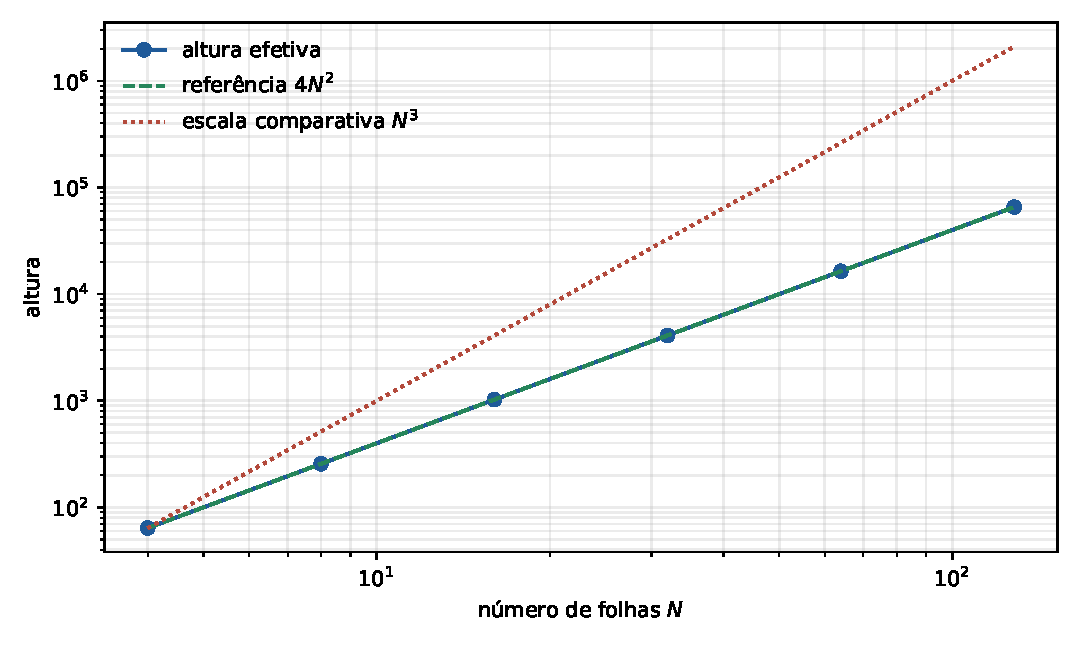
\includegraphics[width=.88\linewidth]{fig_altura_agendas.pdf}
 \caption{A altura efetiva da construção quadrática acompanha $N^2$; a
 curva $N^3$ corresponde ao fator de malha que o denominador comum absorve.}
 \label{fig:height-schedules}
\end{figure}

A \cref{fig:height-schedules} confirma, na construção quadrática auditada, a
separação entre a agenda provada $N^2$ e a escala comparativa $N^3$.

O programa \texttt{espacos\_aproximacao.py} usa
\texttt{fractions.Fraction} para reconstruir todos os valores nodais,
parâmetros, alturas e erros quadráticos. Ele verifica ainda, por enumeração
de $\mathcal Q_H$, a igualdade \eqref{eq:arithmetic-floor}; reproduz a
altura geométrica mínima $H=N$ das malhas uniformes em $[0,1]$; registra o
teste integral da série logarítmica; e emite o certificado simbólico da
\cref{prop:nonhomogeneous-functional}. Os testes são executados
independentemente da programação dinâmica das
\cref{sec:fixed-dp,sec:variable-dp}.
